%%%%%%%%%%%%%%%%%%%%%%%%%%%%%%%%%%%%%%%%%
% Thin Sectioned Essay
% LaTeX Template
% Version 1.0 (3/8/13)
%
% This template has been downloaded from:
% http://www.LaTeXTemplates.com
%
% Original Author:
% Nicolas Diaz (nsdiaz@uc.cl) with extensive modifications by:
% Vel (vel@latextemplates.com)
%
% License:
% CC BY-NC-SA 3.0 (http://creativecommons.org/licenses/by-nc-sa/3.0/)
%
%%%%%%%%%%%%%%%%%%%%%%%%%%%%%%%%%%%%%%%%%

%----------------------------------------------------------------------------------------
%	PACKAGES AND OTHER DOCUMENT CONFIGURATIONS
%----------------------------------------------------------------------------------------

\documentclass[a4paper, 11pt]{article} % Font size (can be 10pt, 11pt or 12pt) and paper size (remove a4paper for US letter paper)

\usepackage[protrusion=true,expansion=true]{microtype} % Better typography

\usepackage{graphicx} % Required for including pictures
\graphicspath{ {screenshots/} }

\usepackage{wrapfig} % Allows in-line images
\usepackage{listings}

\usepackage{mathpazo} % Use the Palatino font
\usepackage[T1]{fontenc} % Required for accented characters
\linespread{1.05} % Change line spacing here, Palatino benefits from a slight increase by default

\makeatletter
\renewcommand\@biblabel[1]{\textbf{#1.}} % Change the square brackets for each bibliography item from '[1]' to '1.'
\renewcommand{\@listI}{\itemsep=0pt} % Reduce the space between items in the itemize and enumerate environments and the bibliography

\renewcommand{\maketitle}{ % Customize the title - do not edit title and author name here, see the TITLE block below
\begin{flushright} % Right align
{\LARGE\@title} % Increase the font size of the title

\vspace{50pt} % Some vertical space between the title and author name

{\large\@author} % Author name
\\\@date % Date

\vspace{40pt} % Some vertical space between the author block and abstract
\end{flushright}
}

%----------------------------------------------------------------------------------------
%	TITLE
%----------------------------------------------------------------------------------------

\title{\textbf{Skipping the textures}\\ % Title
Computer Graphics final assignment} % Subtitle

\author{\textsc{David Kleingeld} % Author
\\{\textit{Leiden University}}} % Institution

\date{\today} % Date

%----------------------------------------------------------------------------------------

\begin{document}

\maketitle % Print the title section

%----------------------------------------------------------------------------------------
%	ABSTRACT AND KEYWORDS
%----------------------------------------------------------------------------------------

%\renewcommand{\abstractname}{Summary} % Uncomment to change the name of the abstract to something else

\begin{abstract}
Morbi tempor congue porta. Proin semper, leo vitae faucibus dictum, metus mauris lacinia lorem, ac congue leo felis eu turpis. Sed nec nunc pellentesque, gravida eros at, porttitor ipsum. Praesent consequat urna a lacus lobortis ultrices eget ac metus. In tempus hendrerit rhoncus. Mauris dignissim turpis id sollicitudin lacinia. Praesent libero tellus, fringilla nec ullamcorper at, ultrices id nulla. Phasellus placerat a tellus a malesuada.
\end{abstract}

\hspace*{3,6mm}\textit{Keywords:} lorem , ipsum , dolor , sit amet , lectus % Keywords

\vspace{30pt} % Some vertical space between the abstract and first section

%----------------------------------------------------------------------------------------
%	ESSAY BODY
%----------------------------------------------------------------------------------------

\section*{Introduction}
Here we try to render a basic landscape without using textures. Our program can be devided into the following sections: SDLApp: containing userinput and main loop, Logic: containing the rendering and movement code and support files: handling png decode, math and shaders. Most of the code base is derived from the computer grapshics hightmap workshop.

Most computer graphics programs make use of textures to apply color to the vertices. Textures are arrays of colors that are applied to 3d models by the gpu. One of the major advantages of using textures is that they allow more that 2 colors between vertices. Imagine a simple tent with 2 tent poles, here each end of the sheet would be a vertex. For each vertex we would be able to specify the color. In between the vertices the gpu interpolates the color. In the tent anology that means we are be able to pour a bucket of paint over each end of the sheet. We cant put more detail in. Using a texture however we can specify the colors between the vertices, this is like painting on the tent sheets.

Why the would we try to work without textures? Simple, to use a texture we need to know where the tent poles fit under the sheet. In other words we need to map the vertices to parts of the texture. This is hard work. It also limits, or greatly complicates the editing of colors from the program.

By using more vertices we can put in the same amount of detail as using a texture but at a cost of performance.
%------------------------------------------------

\section*{Difficulties}

There where 2 major hurdles in this project: Creating a manuverable camera and mapping colors to vertices from files. The camera is needed to check if the colors are applied to the vertices as intended. It was however a challange connecting the linear algebra behind the required transformation to the existing code base.

The hardest problem was mapping the colors to the vertices correctly. We loaded in a png image and splitting it into rgb float arrays. Then we extended the loadterrain function to correctly set the color information. However once this was send to the gpu this resulted in a strange color pattern. Clearly te colors where applied to the wrong vertices. Eventually we found the ommission of 'glBindAttribLocation' was the cause. Though not needed for the position and normal shader variables omitting to set the attribute location for the color information caused the latter to be interperted in a wrong order.

Thus changing the shaderloading function from:
\begin{lstlisting}
	p = glCreateProgram();
	glAttachShader(p, vs);
	glAttachShader(p, fs);
	glLinkProgram(p);
\end{lstlisting}

to:
\begin{lstlisting}
	p = glCreateProgram();
	glAttachShader(p, vs);
	glAttachShader(p, fs);

	glBindAttribLocation(p, 0, "in_position");
	glBindAttribLocation(p, 1, "in_normal");
	glBindAttribLocation(p, 2, "in_color");
	glBindAttribLocation(p, 3, "in_waterpos");

	glLinkProgram(p);
\end{lstlisting}
solved the colors being mappend incorrectly.

%------------------------------------------------


\section*{Usage}

\subsection*{compiling}
The project can be compiled using the included makefile. It requires libsdl1.2 dev and libglew-dev to compile.

\subsection*{executing}
To run use 'make run'. The program will take a few seconds to generate vertices from hightmap and pre map colors to the generated vertices. Then the mouse and arrow keys can be used to look and move around the world. The program captures the mouse, it can be released by pressing escape. Then to quit either close the window or press ctrl+c in the terminal.

\subsection*{changing assets}
The hightmap and colormap can be changed by replacing the files colormap.png and heightmap.png in the assets folder. For the heightmap only the red channel is used. Brighter red results in heigher terrain. The default hightmap has a resolution of 1024x1024. The colormap should match these dimensions. Though larger dimensions are supported it is not recommended as the number of generated vertices will become to high to render smoothly.

\section*{Conclusion}

Though simple and instructive we do not recommend this method. To get any amount of detail you require a large amount of different colors and thus vertices. This results in a lot of textices that do not change the geometry but do tax performance. This neglects that geometry is often implied using colors, think about darker areas between objects implying the objects are popping out. Using this you need a less complicated 3d model to get the same appearend detail. This is not an option while using vertices for coloring.

\section*{References}

%----------------------------------------------------------------------------------------
%	BIBLIOGRAPHY
%----------------------------------------------------------------------------------------

\bibliographystyle{unsrt}

\bibliography{sample}

%----------------------------------------------------------------------------------------

\section*{Screenshots}


\begin{figure}[ht]
\caption{image of a flat area while showing a wire frame on top}
\centering
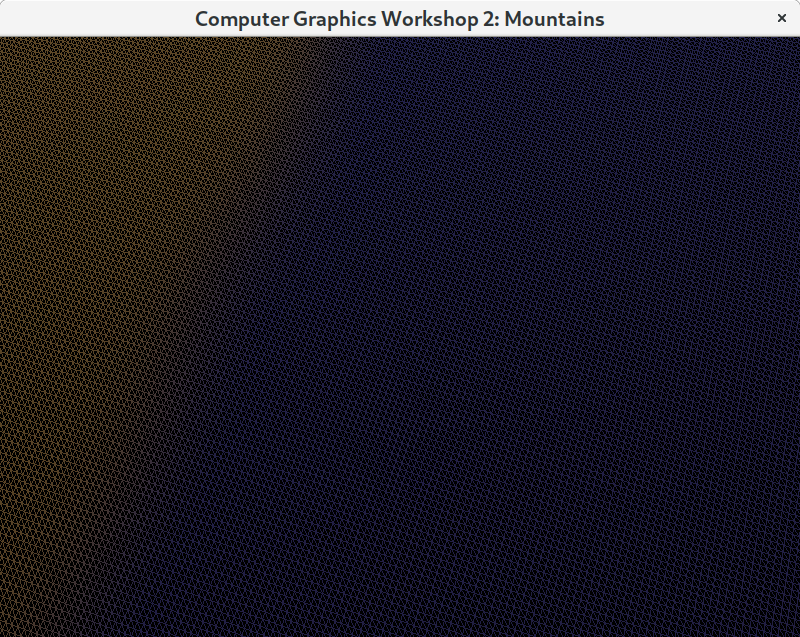
\includegraphics[width=0.5\textwidth]{wire_frame}
\end{figure}



\begin{figure}[ht]
\caption{top down view showing the gradient}
\centering
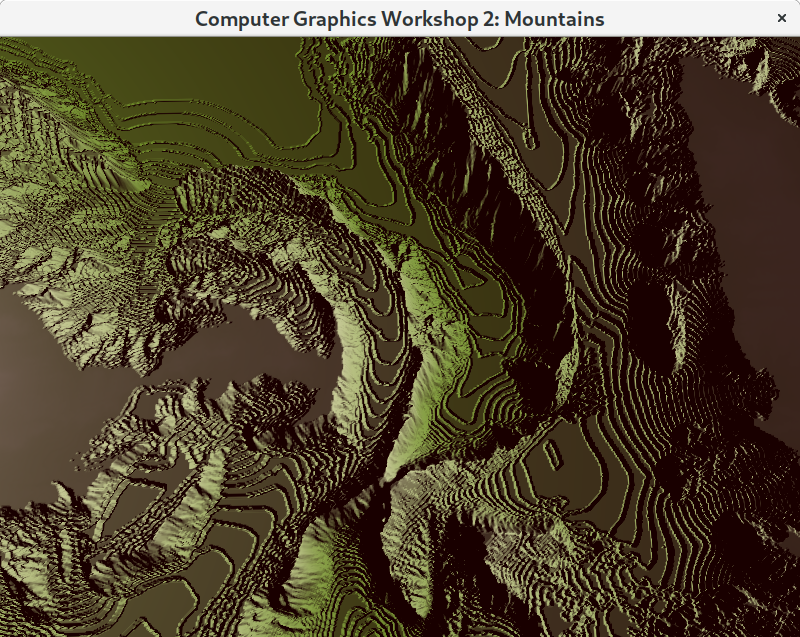
\includegraphics[width=0.5\textwidth]{down_view}
\end{figure}



\begin{figure}[ht]
\caption{shows the details in the landscape at some distance}
\centering
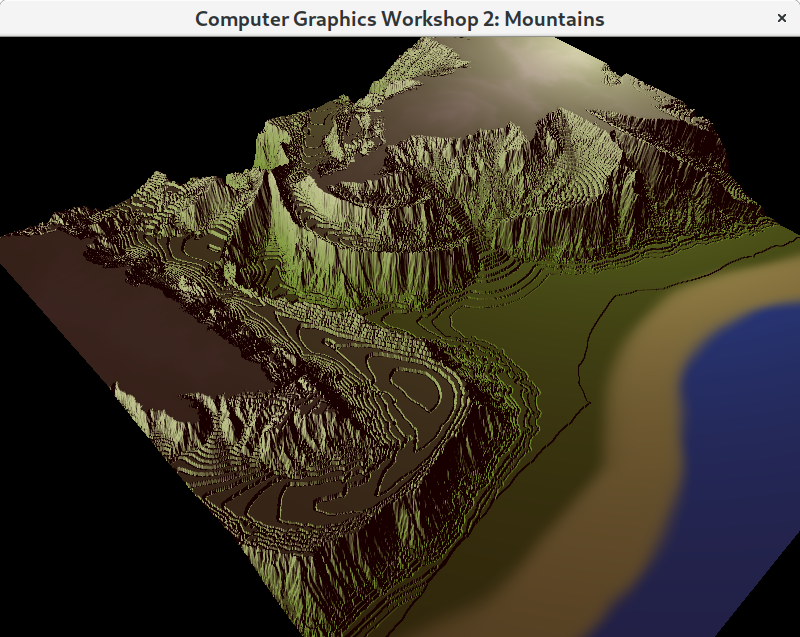
\includegraphics[width=0.5\textwidth]{landscape}
\end{figure}



\begin{figure}[ht]
\caption{closeup showing low appearent geometry resolution}
\centering
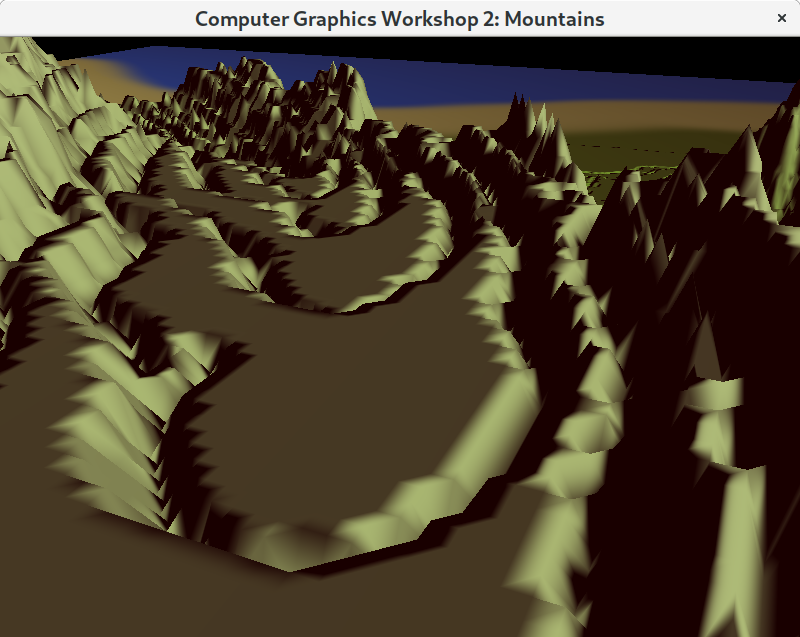
\includegraphics[width=0.5\textwidth]{shows_gradient}
\end{figure}



\begin{figure}[ht]
\caption{showing the side of the terrain}
\centering
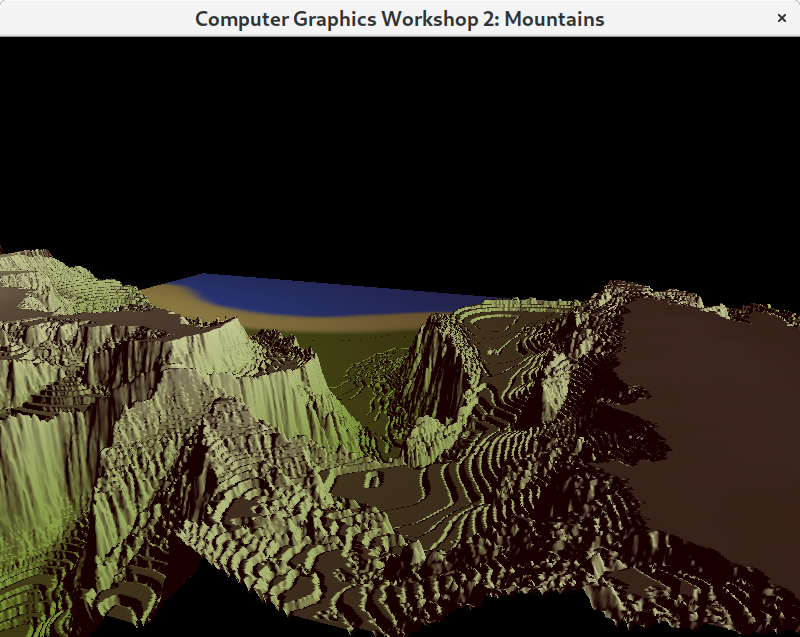
\includegraphics[width=0.5\textwidth]{side_view}
\end{figure}




\end{document}